%particles
\newcommand{\jpsi}{\rm J/$\psi$}
\newcommand{\psip}{$\psi^\prime$}
\newcommand{\jpsiDY}{\rm J/$\psi$\,/\,DY}
\newcommand{\chic}{$\chi_{\rm c}$}
\newcommand{\pip}{$\pi^{+}$}
\newcommand{\pim}{$\pi^{-}$}
\newcommand{\pizero}{$\pi^{0}$}
\newcommand{\kap}{K$^{+}$}
\newcommand{\kam}{K$^{-}$}
\newcommand{\pbar}{$\rm\overline{p}$}
\newcommand{\ccbar}{\ensuremath{\mathrm{c\overline{c}}}}
\newcommand{\bbbar}{\ensuremath{\mathrm{b\overline{b}}}}
\newcommand{\Dzero}{\ensuremath{\mathrm{D^{0}}}}
\newcommand{\Dzerobar}{\ensuremath{\mathrm{\overline{D}^{0}}}}
\newcommand{\Dpm}{\ensuremath{\mathrm{D^{\pm}}}}
\newcommand{\Ds}{\ensuremath{\mathrm{D_{s}^{\pm}}}}
\newcommand{\Dstar}{\ensuremath{\mathrm{D^{*\pm}}}}

%collision systems
\newcommand{\pp}{pp}
\newcommand{\pPb}{p--Pb}
\newcommand{\PbPb}{Pb--Pb}

%detectors
\newcommand{\ezdc}{$E_{\rm ZDC}$}

%units
\newcommand{\GeVc}{GeV/$c$}
\newcommand{\GeVcsq}{GeV/$c^2$}

%others
\newcommand{\degree}{$^{\rm o}$}
\newcommand{\s}{\ensuremath{\sqrt{s}}}
\newcommand{\snn}{\ensuremath{\sqrt{s_{\rm NN}}}}
\newcommand{\y}{\ensuremath{y}}
\newcommand{\pt}{\ensuremath{p_{\rm T}}}
\newcommand{\dedx}{d$E$/d$x$}
\newcommand{\dndy}{d$N$/d$y$}
\newcommand{\dndydpt}{${\rm d}^2N/({\rm d}y {\rm d}p_{\rm t})$}
\newcommand{\zpar}{\ensuremath{z_{||}}}
\newcommand{\zpargen}{\ensuremath{z_{||}^{\mathrm{part}}}}
\newcommand{\zpardet}{\ensuremath{z_{||}^{\mathrm{det}}}}
\newcommand{\ptchjet}{\ensuremath{p_{\mathrm{T,ch\, jet}}}}
\newcommand{\ptjet}{\ensuremath{p_{\mathrm{T,jet}}}}
\newcommand{\ptchjetgen}{\ensuremath{p_{\mathrm{T,ch\,jet}}^{\mathrm{part}}}}
\newcommand{\ptchjetdet}{\ensuremath{p_{\mathrm{T,ch\,jet}}^{\mathrm{det}}}}
\newcommand{\ptd}{\ensuremath{p_{\mathrm{T,D}}}}
\newcommand{\ptdgen}{\ensuremath{p_{\mathrm{T,D}}^{\mathrm{part}}}}
\newcommand{\ptddet}{\ensuremath{p_{\mathrm{T,D}}^{\mathrm{det}}}}
\newcommand{\antikt}{anti-\ensuremath{k_{\mathrm{T}}}}
\newcommand{\Antikt}{Anti-\ensuremath{k_{\mathrm{T}}}}
\newcommand{\kt}{\ensuremath{k_{\mathrm{T}}}}
\newcommand{\pthard}{\ensuremath{p_{\mathrm{T,hard}}}}
\documentclass[12pt, a4paper, twoside, titlepage]{article}
% font size could be 10pt (default), 11pt or 12 pt
% paper size coulde be letterpaper (default), legalpaper, executivepaper,
% a4paper, a5paper or b5paper
% side coulde be oneside (default) or twoside 
% columns coulde be onecolumn (default) or twocolumn
% graphics coulde be final (default) or draft 
%
% titlepage coulde be notitlepage (default) or titlepage which 
% makes an extra page for title 
% 
% paper alignment coulde be portrait (default) or landscape 
%
% equations coulde be 
%   default number of the equation on the rigth and equation centered 
%   leqno number on the left and equation centered 
%   fleqn number on the rigth and  equation on the left side
%
\usepackage{hyperref}
\usepackage{graphicx}  % needed for figures
\usepackage{dcolumn}   % needed for some tables
\usepackage{bm}        % for math
\usepackage{amssymb}   % for math
\usepackage{amsfonts}
\usepackage{amsmath}
\usepackage{graphics}
\usepackage{grffile}   % to handle dots in graphics file names
\usepackage{epsfig}
\usepackage{units}
\usepackage{comment}
\usepackage[usenames]{color}
\usepackage[normalem]{ulem} % for strikethroughs (\sout{})
\usepackage{color}
\usepackage[utf8]{inputenc}
\usepackage[T1]{fontenc}
\usepackage{subfigure}
\usepackage{multirow}
\usepackage{tablefootnote}
\usepackage{bm}
\usepackage[numbers,sort&compress]{natbib}
\title{Measurement of charm jet cross-sections and fragmentation functions
with the ALICE detector at the LHC}
\author{Salvatore Aiola  \\
	Advisers: John Harris, Helen Caines \\
	Yale University Physics Department
	}

\date{\today} 
% \date{\today} date coulde be today 
% \date{25.12.00} or be a certain date
% \date{ } or there is no date 
\begin{document}
% Hint: \title{what ever}, \author{who care} and \date{when ever} could stand 
% before or after the \begin{document} command 
% BUT the \maketitle command MUST come AFTER the \begin{document} command! 
\maketitle

\begin{abstract}
The measurement of the charm production cross section in \pp\ collisions is an important, sensitive, test of perturbative Quantum Chromo-Dynamics (pQCD) calculations.
It is also an ideal probe of the hot and dense medium, known as the Quark-Gluon Plasma (QGP), produced in ultra-relativistic heavy-ion collisions.
The charm production cross section is also relevant for high-energy neutrino astrophysics, where neutrinos coming from the decay of charmed hadrons produced
in cosmic-ray atmospheric showers are one of the largest sources of background.

Charm quarks are produced abundantly at the CERN Large Hadron Collider (LHC). The ALICE experiment is specifically endowed with the tools for measuring
jets originating from charm quarks in the low momentum region, thanks to its Particle Identification (PID) capabilities and good momentum resolution.
The measurement of the charm jet cross section and of the internal properties of charm jets, particularly the fragmentation function, will result in an important
contribution to the advancement of the related subfields: perturbative QCD theory and phenomenology, QCD at high temperature (QGP), neutrino astrophysics.
\end{abstract}

\tableofcontents % create a table of contents 
\newpage

\section{Introduction}
The \emph{charm} quark was discovered in 1974 almost simultaneously by two groups, working at SLAC~\cite{Richter:1974} and at BNL~\cite{Ting:1974}.
The two groups observed a new resonance with a mass of about 3.1 \GeVcsq\ decaying into a pair of leptons.
The decay width was measured to be smaller than 1.3 MeV~\cite{Richter:1974}; this feature
was in itself a strong indication of the existence of a new quantum number, conserved by strong nuclear interactions 
but violated in electro-weak processes.
This resonance later became known with the double name \jpsi\ and was identified as one of the possible bound states
of a new heavier quark, \emph{charm}, and of its corresponding anti-quark~\cite{Appelquist:1975, DeRujula:1975}. 
\begin{comment}
A few years later (1977) an even heavier quark, the \emph{bottom} quark,
was discovered~\cite{Lederman:1977}; the sixth and last known quark, \emph{top}, took a bit longer (1995), due to its comparatively huge mass of about 173 \GeVcsq~\cite{CDF:1995,D0:1995}.
\end{comment}

\begin{figure}[tbh]
\begin{center}
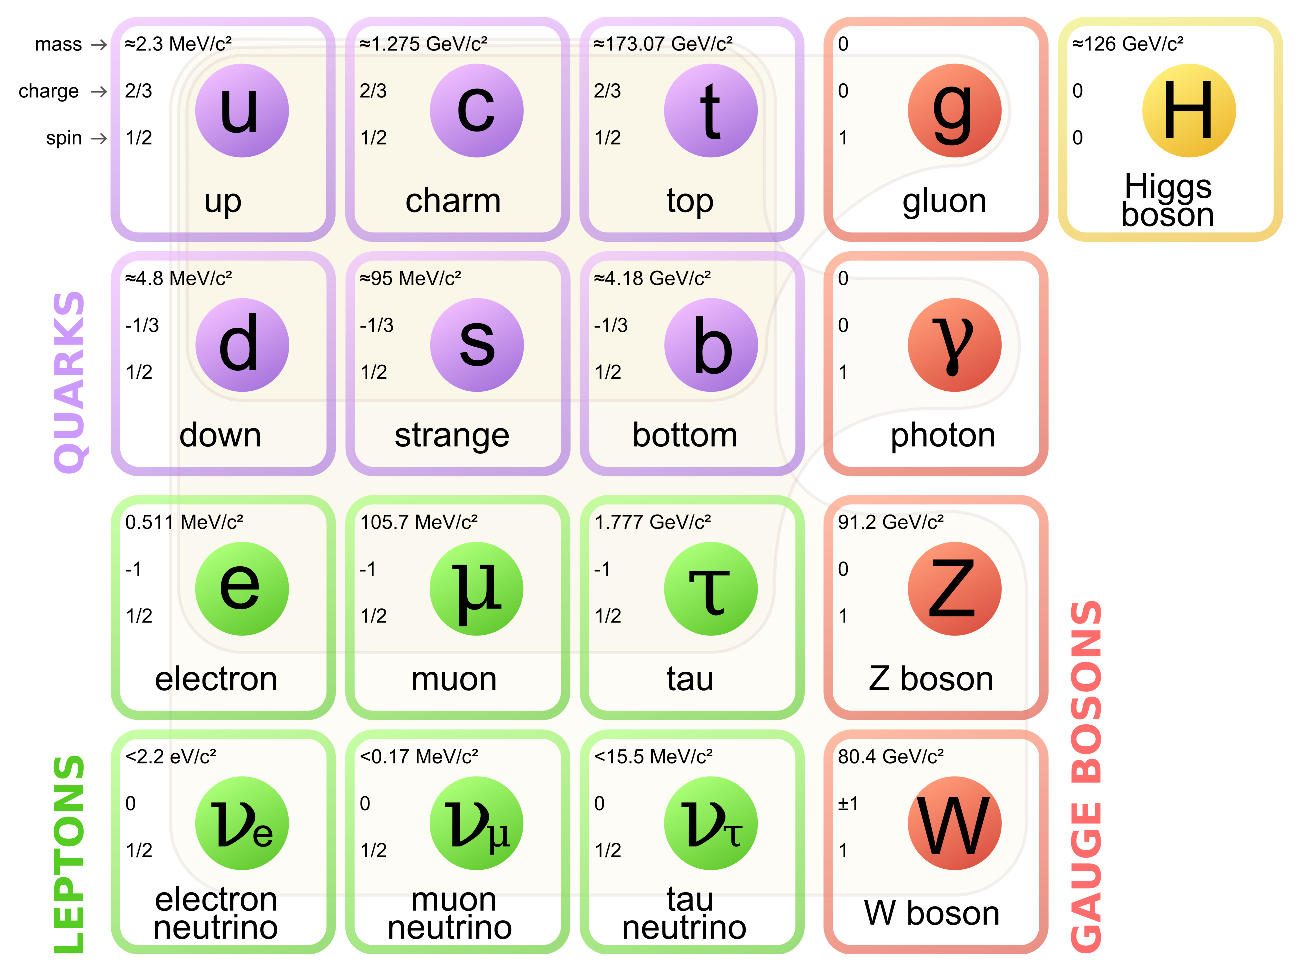
\includegraphics[width=0.8\textwidth]{img/standard_model}
 \caption{Standard Model of Particle Physics~\cite{Wikipedia:StandardModel}.} 
 \label{fig:standard_model}
\end{center}
\end{figure}
Figure~\ref{fig:standard_model} shows an illustration of the Standard Model, which includes
3 generations of leptons (electron, muon, tau), 3 generations of quarks, 4 interaction bosons, ($\gamma$, Z, $\mathrm{W}^{\pm}$, g) and the Higgs boson
recently observed by the ATLAS and CMS Collaborations \cite{ATLAS:2012b,CMS:2012d}.
Each generation of particles (either quarks or leptons) differs from the others in the strength of its coupling to the Higgs boson,
which results in different observed masses.

At hadron colliders, charm quarks are produced as a result of a hard scattering of partons. Like lighter quarks or gluons, charm quarks
fragment into collimated sprays of hadrons called \emph{jets}. The charm content of the jet is conserved throughout the fragmentation process,
which is dominated by Quantum Chromo-Dynamics (QCD), the theory of strong nuclear interactions.
The charm content of a jet can be identified by looking for the presence of charmed hadrons, i.e. hadrons that have
a charm quark among their valence quarks. Since all charmed hadrons have short lifetimes ($\tau \lesssim 10^{-12}$~s) their presence is inferred
using a combination of Particle Identification (PID) techniques and selection of specific kinematics and topological patterns of their decay products.

The production cross-section of charm jets is significantly smaller than the ones of lighter quarks or gluons. The internal
properties of the jets are also affected due to the heavier mass of the originating parton, 
in particular the fragmentation is expected to be harder for charm jets.

\begin{figure}[tbh]
\begin{center}
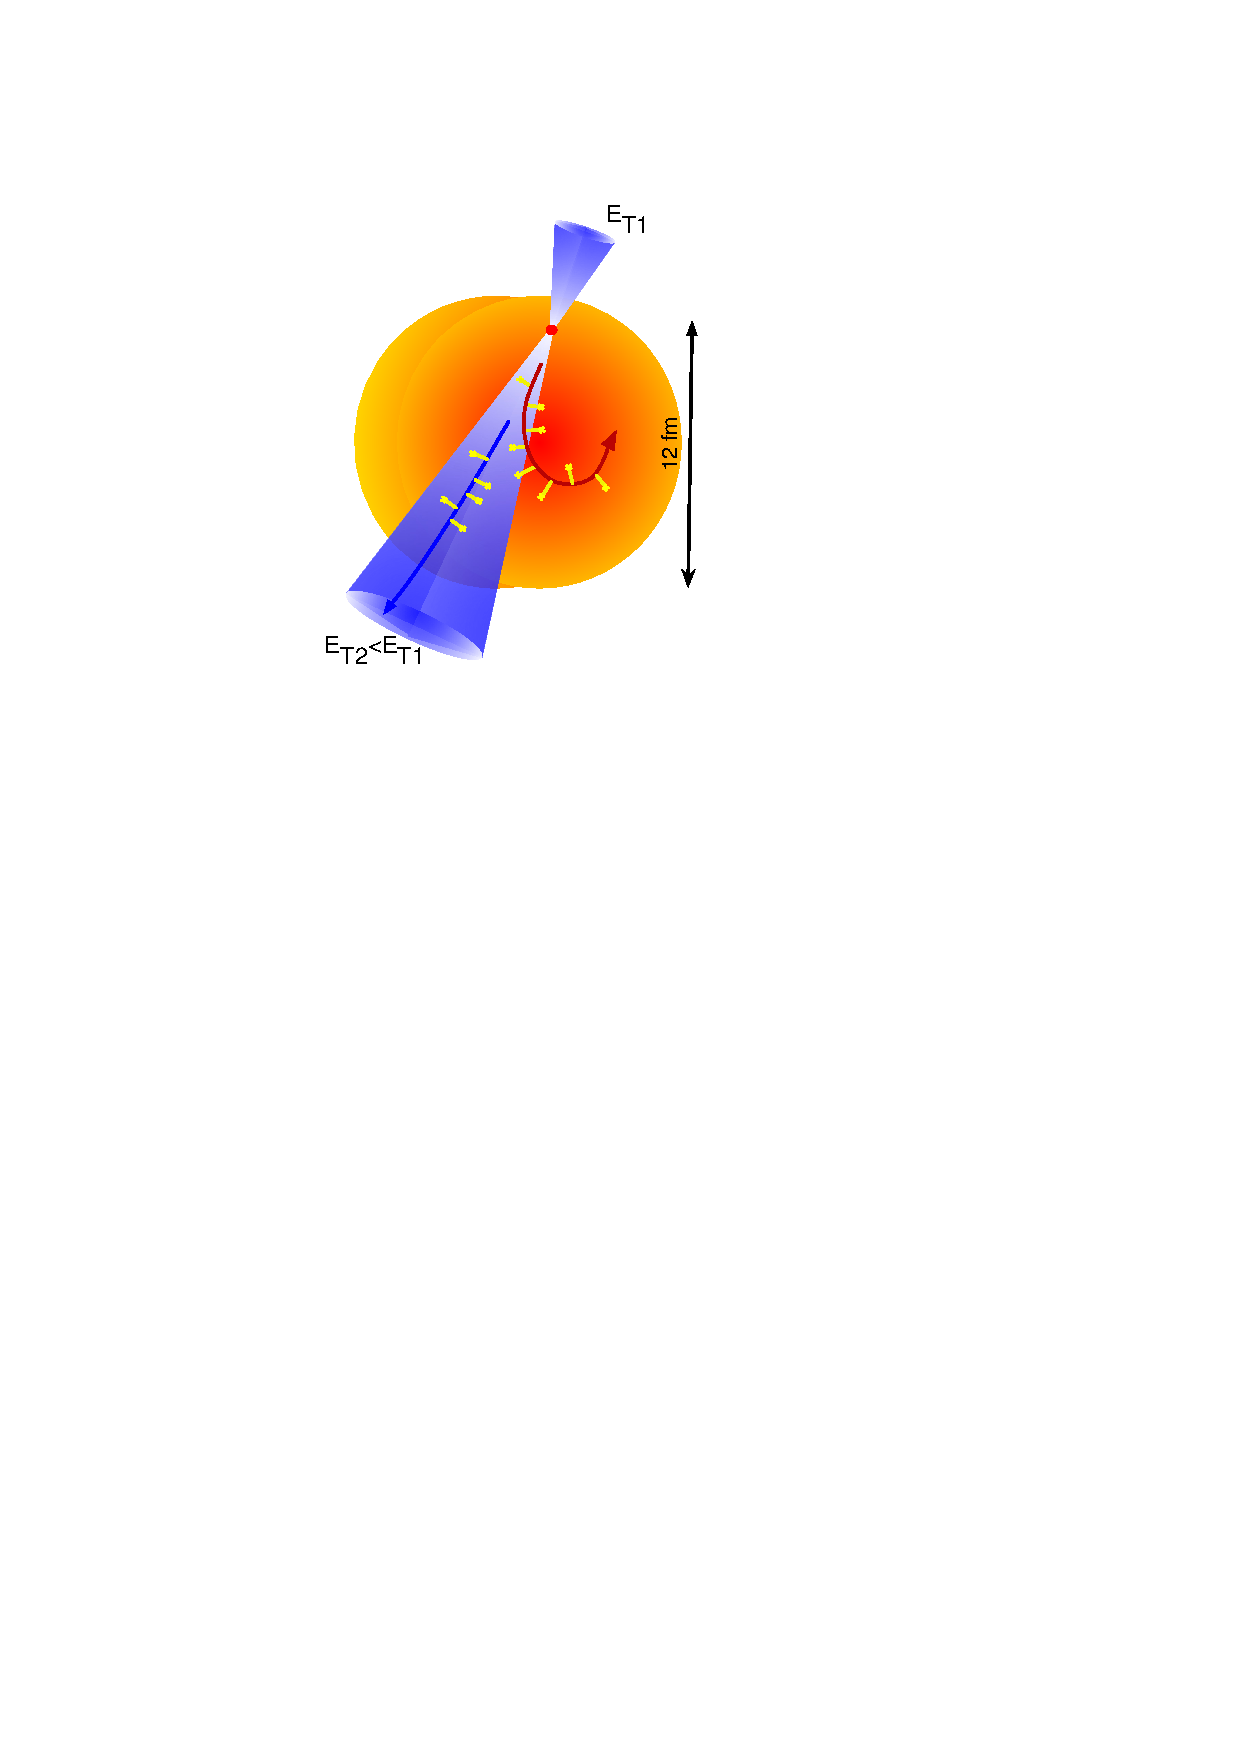
\includegraphics[width=0.5\textwidth]{img/jetquenching}
 \caption{Hard scattered partons interact with the QGP generated in ultra-relativistic heavy-ion collisions.} 
 \label{fig:jetquenching}
\end{center}
\end{figure}
Heavy quarks are also an ideal probe of the hot and dense matter, known as the Quark-Gluon Plasma (QGP)~\cite{STAR:2005a, PHENIX:2005a, ALICE:2010b, ALICE:2011b, CMS:2013d, ATLAS:2013c}, 
that is created in ultra-relativistic heavy-ion collisions. 
Hard scattered partons, including heavy quarks, are produced early in the collision. They interact with the QGP, which increases their virtuality and interferes with the
parton fragmentation process as depicted in Fig.~\ref{fig:jetquenching}. 
This effect, known as \emph{jet quenching}, can lead to a suppression of the jet yield, the disappearance of the back-to-back jet correlation peak,
and a broadening and softening of the jet fragmentation. 
A number of experimental results consistent with jet quenching have been reported in last decade~\cite{PHENIX:2003a, PHENIX:2008b, STAR:2003b, STAR:2003c, STAR:2006a, ALICE:2010d, CMS:2011c, CMS:2012b, ATLAS:2014d, ALICE:2015a}.
High-energy charm jets behave very much like jets that originate from light quarks; however at lower energies, comparable to the charm quark mass, the charm quark is expected
to interact less strongly with the QGP, a phenomenon known as the dead-cone effect~\cite{Dokshitzer:2001}.

Charm quarks are produced abundantly at the Large Hadron Collider, which provides \pp, \pPb\ and \PbPb\ collisions at unprecedented high collision energies and luminosities.
At the LHC, the PID and low-momentum tracking capabilities are among the strongest points of ALICE~\cite{ALICE:2014b}.
Especially vertexing, tracking and PID are crucial to efficiently identify the decay products of charmed hadrons; tracking and calorimetry are used together to reconstructed the energy flow from which jets can be identified.
ALICE is very well suited to perform a precise measurement of charm jets in a (mostly) unexplored kinematical region, i.e. low and intermediate momentum charm jets. Furthermore, the performance of ALICE
is optimized for heavy-ion collisions, where charm jet measurements can provide important insights about the QGP.

\section{The Large Hadron Collider}
The \emph{Large Hadron Collider} (LHC) at CERN is the world's largest particle collider ever built.
It is housed in a tunnel with a circumference of 27 km, between 50 and 175 m beneath
the France-Switzerland border near the city of Geneva. The tunnel was built in the 1980s and was used until 
the late 1990s to house the Large Electron-Positron Collider (LEP). The construction of the LHC took about 10 years and started
during the decommissioning phase of LEP. 

Two parallel beam pipes run through the tunnel,
through which particles travel in opposite directions, intersecting at four points where four different experiments
detect and measure the collisions (\mbox{ALICE}, \mbox{ATLAS}, \mbox{CMS}, \mbox{LHCb}). More than 1,000 superconducting dipole magnets
are used to keep the particles in their circular trajectories, plus approximately 400 superconducting quadrupole and higher multipole
magnets, which are needed to keep the beams focused and provide other optical corrections.

Protons and lead ions undergo several pre-acceleration steps before being injected into the LHC at an energy of 900 GeV (355 GeV per nucleon for lead ions).
They are injected in bunches, spaced by 25 ns (or multiple thereof) for a maximum of 2,808 bunches when operating at full luminosity in \pp\ collision mode.
Acceleration is provided through radio frequency cavities. At its highest energy (currently 6.5 TeV for proton beams) the dipole magnets need to generate
a magnetic field of 7.7 T.

At time of writing (July 2016) the LHC is in its Run-2 phase. The first operational phase of the LHC (Run-1) started in November 2009 and was 
concluded in February 2013. In this first phase the LHC successfully provided \pp, \pPb\ and \PbPb\ collisions.
Between 2013 and 2015 the LHC operations were stopped to allow for upgrades to the machine and to the four experiments (Long Shutdown 1, or LS1).
Run-2 started in April 2015 and is scheduled to extend till the end of 2018. Table~\ref{tab:LHCop} shows details of the LHC operations in Run-1 and Run-2.
After Run-2 another 2-year stop is foreseen (LS2) to allow for more upgrades, before the third operational phase (scheduled to start in 2021).

\begin{table}
\centering
\begin{tabular}[tbh]{lrr}
Collision system	&	Years		&	\s\ (TeV)	\\
\hline
\hline
\\
\multicolumn{3}{l}{Run-1} \\
\hline
\multirow{4}{*}{\pp}	&	2009			&	0.9		\\
				&	2010, 2011	&	7		\\
				&	2011			&	2.76		\\
				&	2012			&	8		\\
\hline
\PbPb			&	2010, 2011	&	2.76 		\\
\hline
\pPb				&	2012\tablefootnote{Pilot run}, 2013	&	5.02	\\
\hline
\\
\multicolumn{3}{l}{Run-2} \\
\hline
\multirow{2}{*}{\pp}	&	2015, 2016				&	13	\\
				&	2015						&	5.02	\\
\hline
\PbPb			&	2015						&	5.02	\\
\hline
\pPb				&	2016\tablefootnote{Planned for fall 2016}		&	5.02, 8	\\
\hline
\end{tabular}
\caption{LHC Run-1 and Run-2 operations.
\label{tab:LHCop}}
\end{table}
\section{The ALICE Experiment}
ALICE (\emph{A Large Ion Collider Experiment}) is the experiment dedicated to the study of heavy-ion collisions at the LHC.
Figure~\ref{fig:alice} shows a schematic of the ALICE detector.
ALICE is a complex experiment made of several independent detector sub-systems that are operated synchronously.
The main detectors are in the central barrel and cover the mid-rapidity region ($\lvert \eta\rvert \lesssim 1$).
Table~\ref{tab:ALICEdetectors} lists the ALICE detector subsystems
relevant for my dissertation.
A full description of ALICE and of its performance during LHC Run-1 is available at Ref.~\cite{ALICE:2014b}.\

\begin{figure}[tb]
\begin{center}
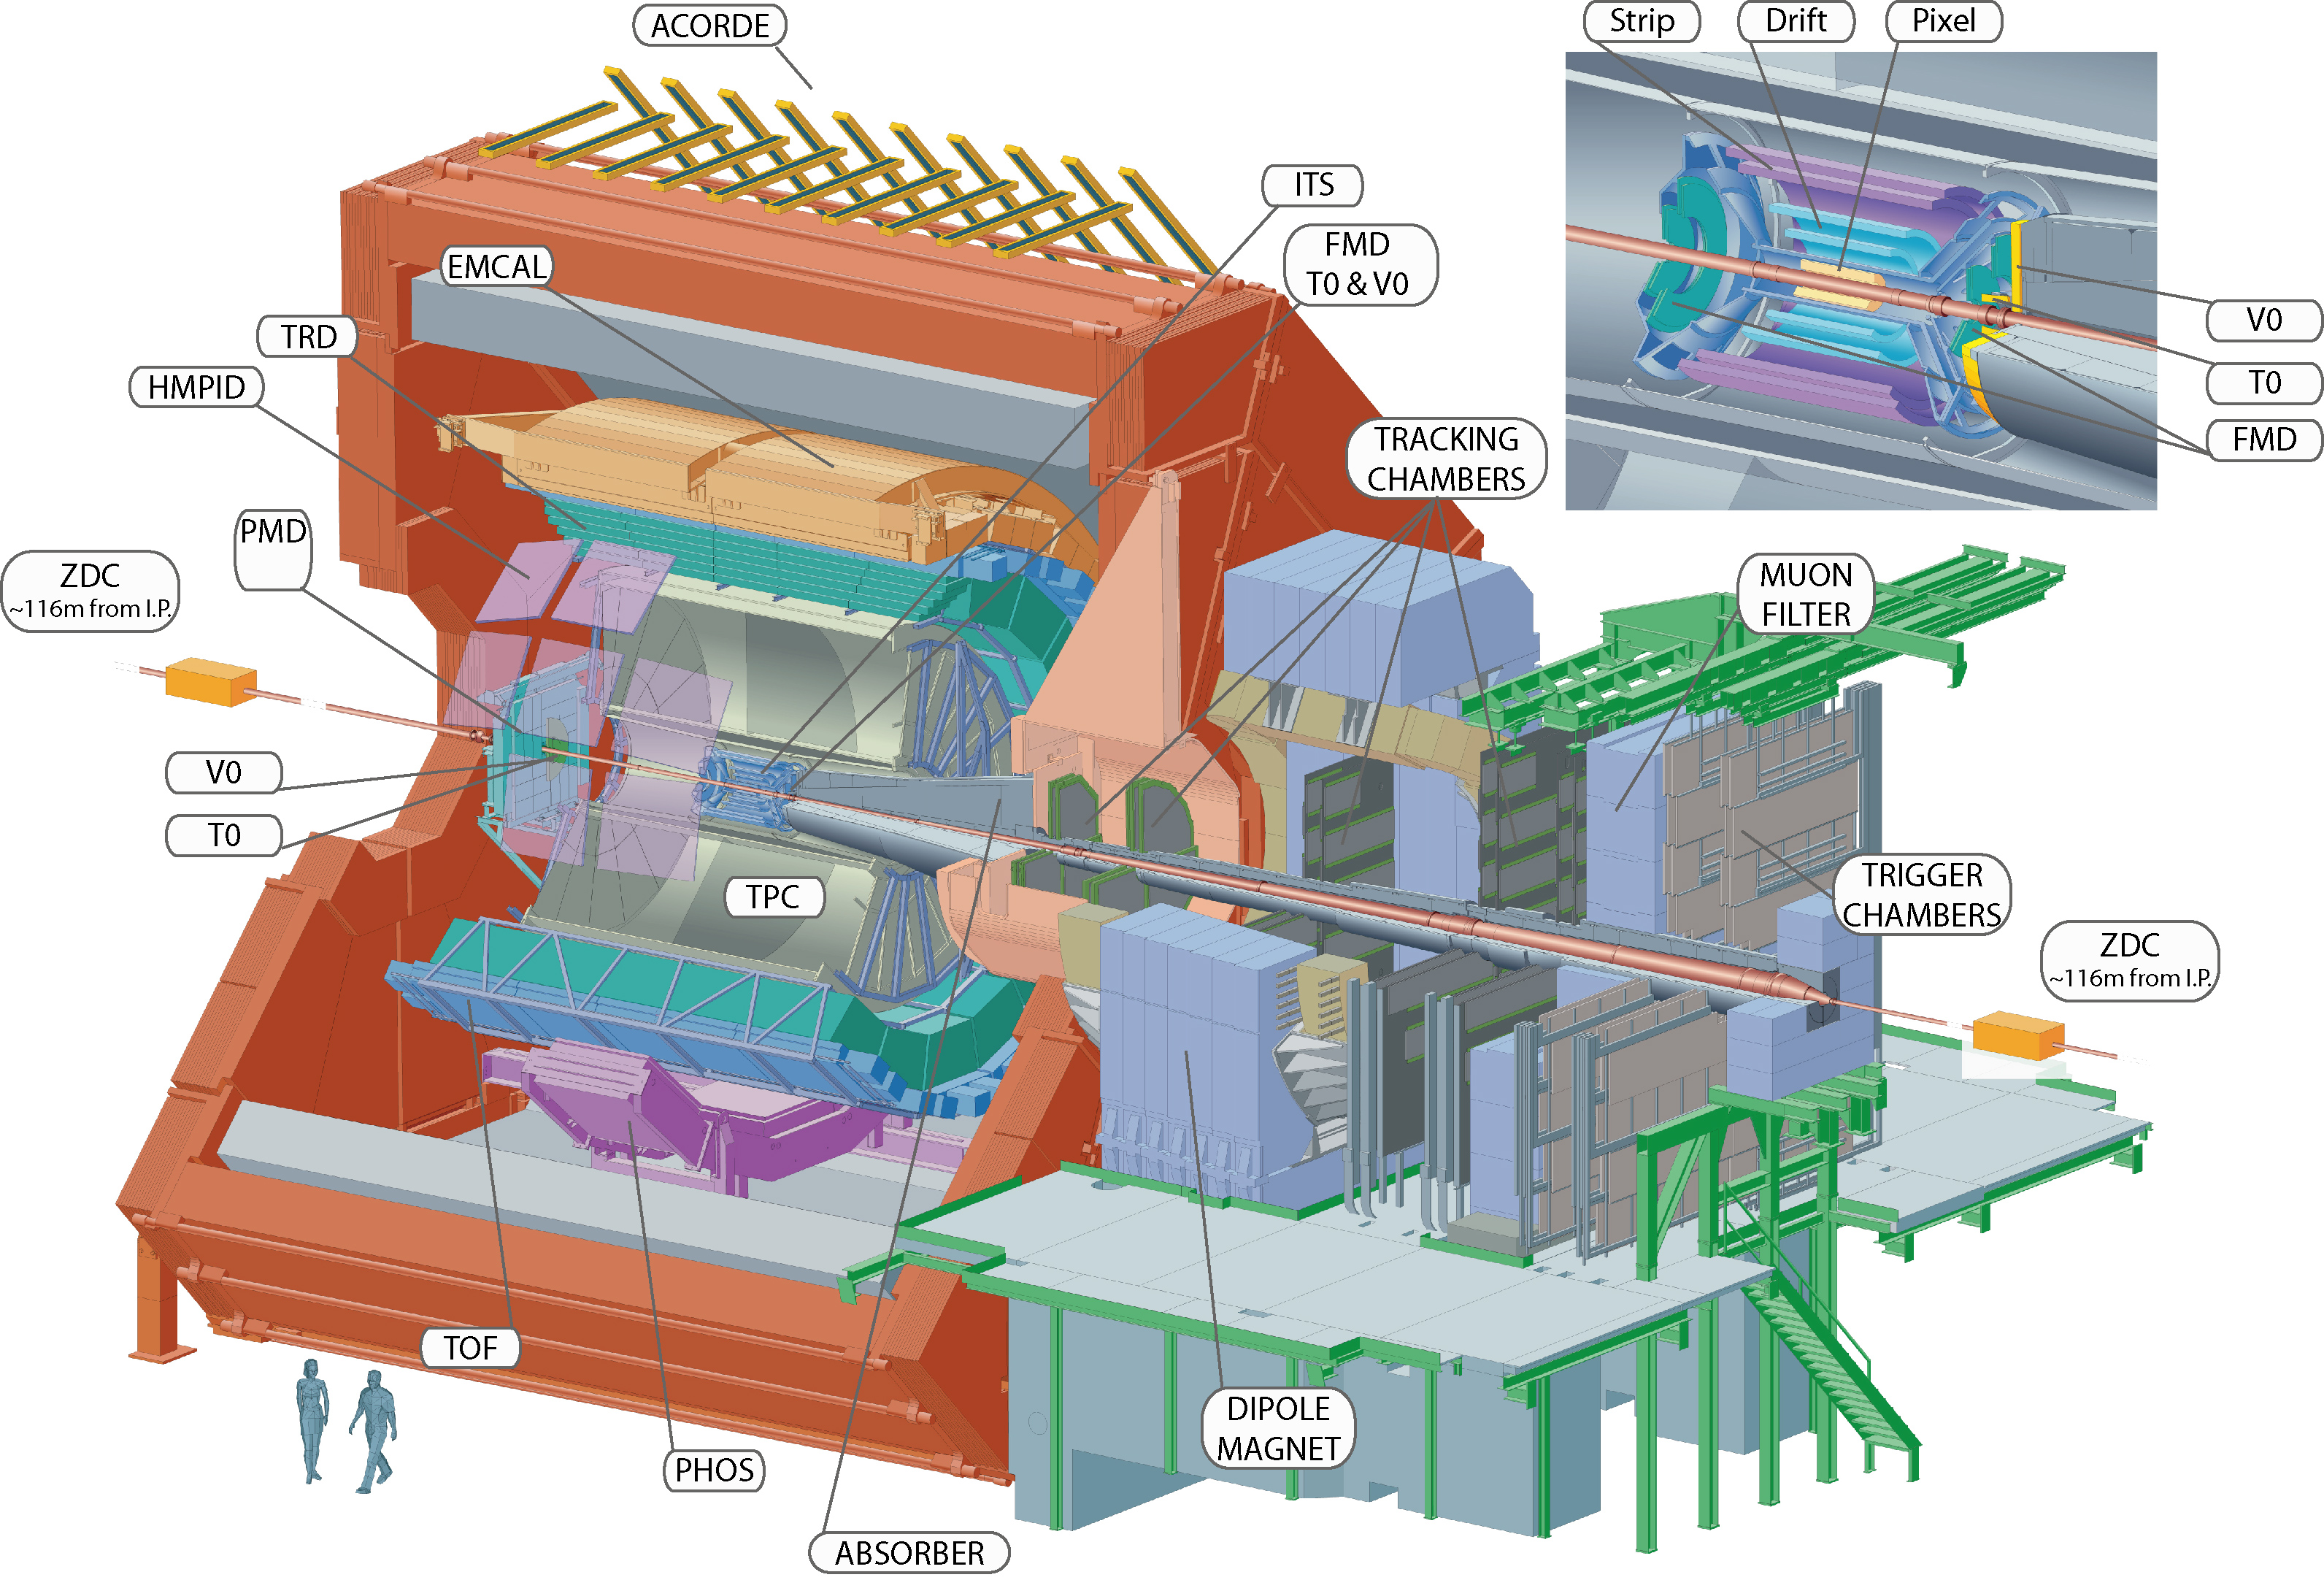
\includegraphics[width=0.7\textwidth]{img/alice}
 \caption{3D ALICE Schematic; central-barrel detectors are visible inside the red solenoid magnet;
 the muon tracking station is on the right side; in the upper-right corner there is a zoomed inlay of the ITS.} 
 \label{fig:alice}
\end{center}
\end{figure}

\begin{table}[bt]
\centering
\begin{tabular}{lcccc}
Detector		& Pseudo-rapidity		& Technology			& Main purpose			\\
\hline 
\hline
\\
SPD			& $\lvert \eta\rvert <2.0$	& Si pixel				& tracking, vertex		\\
SDD			& $\lvert \eta\rvert <0.9$ 	& Si drift				& tracking, PID			\\
SSD			& $\lvert \eta\rvert <1.0$ 	& Si strip				& tracking, PID			\\
TPC 			& $\lvert \eta\rvert <0.9$ 	& gas drift+MWPC		& tracking, PID			\\
TOF			& $\lvert \eta\rvert <0.9$	& MRPC				& PID				\\
EMCal		& $\lvert \eta\rvert <0.7$ 	& Pb+scint. 			& photons and jets		\\
DCal			& $\lvert \eta\rvert <0.7$ 	& Pb+scint. 			& photons and jets		\\
\multirow{2}{*}{V0}& $2.8 <\eta< 5.1$,	&\multirow{2}{*}{scint.}	& trigger, multiplicity,		\\
			& $-3.7 <\eta<-1.7$		&					& vertex				\\
\multirow{2}{*}{T0}& $4.6 <\eta< 4.9$,	&\multirow{2}{*}{quartz}	& trigger, time,			\\
			& $-3.3 <\eta<-3.0$		&					& vertex				\\
\end{tabular}
\caption{List of the ALICE detector subsystems relevant for the D-tagged jet analysis. All detectors listed above have full azimuthal acceptance except EMCal and DCal 
which cover $80^{\circ} <\phi< 187^{\circ}$ and $253^{\circ} <\phi< 320^{\circ}$, respectively.
\label{tab:ALICEdetectors}}
\end{table}
\section{D-tagged jets with ALICE}
\subsection{Physics goals}
The measurement of the charm production cross section in \pp\ collisions is an important sensitive test of perturbative QCD (pQCD) calculations.
At the LHC energies, the measurement of charm production at low \pt\ probes the parton distribution functions (PDFs)
of the proton at small values of parton fractional momentum, $x$, and squared momentum transfer, $Q^2$.
For illustration, using a simplified $2 \rightarrow 2$ kinematics at leading order, c quarks ($m_{\mathrm{c}} \approx 1.5$~\GeVcsq) with
$\pt \sim 2$~\GeVc\ and rapidity $y \sim 0$ probe the parton distribution functions at $x \sim 7 \times 10^{-4}$ and
$Q^2 \sim (5~\mathrm{GeV})^2$.
Perturbative QCD calculations have substantial uncertainties at low \pt, owing to both the large effect of the
choice of the factorization and renormalization scales at low $Q^2$ and to the sizeable uncertainties on the
gluon PDFs at small $x$~\cite{Cacciari:2015}. 

Furthermore, the measurement of the charm cross section in \pp\ collisions provides a baseline to look for collective effects in ultra-relativistic
heavy-ion collisions, particularly the ones related to parton energy loss in the QGP. In this context, another crucial aspect is the precise determination of the
total charm-production cross section, needed to model charmonium regeneration in the QGP~\cite{Zhao:2011}.
Finally, the measurement of the charm differential cross section down to low \pt\ is relevant for cosmic-ray and neutrino
astrophysics: high-energy neutrinos from the decay of charmed hadrons produced in particle showers in the atmosphere constitute an important
background for neutrinos from astrophysical sources~\cite{Gauld:2015, Bhattacharya:2015}.

Most of the charm-related measurements performed at the LHC so far report the production cross section of hadrons
containing heavy quarks~\cite{ALICE:2012d, ALICE:2012e, ATLAS:2012e, LHCb:2013a, ALICE:2014d, ATLAS:2014e, ALICE:2015c, ALICE:2015d, ALICE:2016a, ATLAS:2016a}.
The kinematic properties of jets are closer to those of the originating c quark, when compared to the measurement of the charmed hadrons alone.
Therefore, by measuring the kinematic properties of jets containing heavy-flavor hadrons 
one reduces the dependence on the details of the fragmentation, which is a highly non-perturbative phenomenon, known only with large uncertainties~\cite{dEnterria:2014}.
Furthermore, the details of the charm quark fragmentation can be the subject of a more careful study in which the kinematic observables 
of both the jet and the charmed hadron are available at the same time. In particular the measurement of the fraction of the jet momentum carried 
by the charmed hadron can provide important insights on the charm production mechanism~\cite{CDF:1990, UA1:1990, STAR:2009a, ATLAS:2012d}.

\subsection{Analysis technique}
The analysis relies on the well established D meson reconstruction techniques~\cite{ALICE:2012d, ALICE:2012e, ALICE:2014d, ALICE:2015c, ALICE:2015d, ALICE:2016a}, as well as
jet reconstruction methods~\cite{ALICE:2013c, ALICE:2014a, ALICE:2015e, ALICE:2015f}, both developed by the ALICE Collaboration. In particular I have
contributed significantly to the measurement of jets in \PbPb\ collisions~\cite{ALICE:2015a, Aiola:2013, Aiola:2014} and to the
development and maintenance of the related jet reconstruction software.

Some of the details of the analysis techniques are still under development. In the following section
I will outline the current plan, which may change as the analysis proceeds and more information becomes available.

\subsubsection{Data and event selection}
ALICE has collected data in several collision systems and at different center of mass energies.
Data-taking periods also differ from each other because the conditions of the detector change in time as a result of upgrades,
or subsystem sectors that become inactive or are repaired. The trigger conditions can change as well, depending on the
physics goals set by the Collaboration and on the instantaneous luminosity expected to be delivered by the LHC.
All these factors need to be taken into account when choosing a dataset that best suits a new physics analysis.

I have started to develop my analysis techniques using the data collected by ALICE in 2010 when the LHC was
delivering \pp\ collisions at \s\ = 7 TeV. At that time only 2 EMCal super-modules out of 12 were installed.
This means that the EMCal cannot be used to reconstruct the jet momentum carried by neutral constituents; therefore jets are
reconstructed only using charged particles measured by the central tracking system (TPC and ITS).
Jets reconstructed using only charged particles are referred to as \emph{charged jets}. This dataset is very
well understood within ALICE, in terms of detector performance, and therefore it is a perfect work bench
to test the core analysis techniques without the additional complications coming from using the calorimeter data.
To reconstruct full jets, i.e. jets reconstructed out of charged particles from the tracking system and neutral particles from their
electromagnetic showers in the EMCal-DCal, one has to look at more recent datasets taken with the extended calorimeter acceptance.
The data taken in 2012 with \pp\ collisions at 8 TeV is a very good candidate. Even more interesting could be the data currently (2016)
being collected with \pp\ collisions at 13 TeV.

For the data collected in 2010, only \emph{minimum bias} (MB) triggers were active. These triggers
try to keep the bias coming from online event selection to a minimum, i.e. every time detectors
are exposed to some activity correlated with an LHC bunch crossing, the event is read-out and stored.
The detector sub-systems that are involved in this type of trigger are the SPD, the V0 and the T0.
The data collected in 2012 and the data currently being collected also include triggers
provided by the EMCal-DCal. In particular, a trigger dedicated to jet physics is available for both datasets. 
I have also contributed to the commissioning phase of the 2016 EMCal-DCal trigger earlier this year (see Section~\ref{sect:TriggerCommisioning}).
In this case events are read-out only if a large enough shower has been detected by the calorimeters.
Trigger biases need to be understood and corrected for, using a combination of data-driven methods and simulations.

\subsubsection{Track selection}
For more details about the tracking algorithm used by ALICE see Ref.~\cite{ALICE:2014b}.

Track quality cuts are applied to ensure good momentum resolution. These cuts
depend on the requirements set by a specific physics analysis.
Two types of tracks are used for this analysis. \emph{Global} tracks have the best
momentum and spatial resolution. They include at least one space point in the SPD (first two
layers of the ITS, closer to the beam pipe) and at least a total of three in the whole ITS. They are required also to
match with a track in the TPC, which has to include at least 70 space points and no less than 80\% of the geometrically findable 
space points in the TPC. Decay products of the D mesons are found among this category of tracks.

Due to the non-uniform SPD response, the reconstruction efficiency of the above defined \emph{global} tracks shows a strong azimuthal dependence.
This non-uniform acceptance can interfere with the jet-finding algorithm. To avoid such effects a second type of tracks is added for jet finding.
For this type of tracks the requirement on the SPD is lifted, while keeping all the other requirements unchanged. To improve momentum resolution,
these tracks are constrained to the primary vertex, which is reconstructed using \emph{global} tracks. This track collection is called \emph{hybrid} because
it includes a combination of \emph{global} tracks and \emph{constrained} tracks.

\subsubsection{D meson candidate identification}
ALICE has successfully measured a number of charmed mesons~\cite{ALICE:2012d, ALICE:2012e}.
The \Dzero\ meson has the best signal/background ratio down to low momentum and
is also the most abundant. The \Dzero\ has a mass $m=1.865$~\GeVcsq\ and a mean lifetime $\tau=4.101 \times 10^{-13}$~s.
It is identified through its hadronic decay: \Dzero $\rightarrow$ \pip \kam. The branching ratio of this decay
is relatively small, BR(\Dzero $\rightarrow$ \pip \kam) = 3.88\%~\cite{PDG:2014}. Both the \Dzero\ and its
anti-particle $\overline{\Dzero}$~are considered.

The first step of the analysis is to select events that contain at least one \Dzero\ meson candidate.
\Dzero\ meson candidates are identified looking for opposite-sign track pairs (\emph{daughters}) among all reconstructed \emph{global} tracks.
In order to suppress the background from combinatorial matches, topological and PID cuts are applied.
The topological cuts select pairs that form a \emph{secondary vertex} displaced from the reconstructed
primary vertex. 
PID information on the \Dzero\ candidate daughters is used to reject pairs that do not satisfy the requirement of being a pion-kaon pair.

The pairs that pass the selections are then used in the next steps.
The four-momentum of the \Dzero\ candidate is calculated summing the four-momenta of the two daughters.
When available, PID is used to assign mass values to the \Dzero\ candidate daughters. When PID is not conclusive,
the pair is used twice with either mass combinations (\pip \kam or \pim \kap). Using the four-momentum of the \Dzero\ candidate
the \emph{invariant mass} is calculated according to the usual special relativity formula: $m^2 = E^2 - \bm{p}^2$.

\subsubsection{Jet reconstruction}
For each \Dzero\ candidate a set of particle four-momenta is prepared and fed as input for the jet-finding algorithm.
This set includes the four-momentum of the \Dzero\ candidate and all reconstructed \emph{hybrid} tracks,
excluding the two daughters of the \Dzero. The jet-finding algorithm returns a set of jet candidates, with the particle constituents
assigned to each jet. The jet containing the \Dzero\ candidate can thus be identified and associated with the \Dzero\ candidate for the next steps.

For this analysis I use the \antikt\ algorithm~\cite{Cacciari:2008c}, widely used at the LHC.

Initially I will focus on using only tracks of charged particles for jet reconstruction. Since they miss the momentum
fraction carried by neutral particles, the kinematics of charged jets is less tightly correlated with the kinematics
of the original parton and depends more strongly on the jet fragmentation; however charged jets have also a number advantages
and have been the subject of recent theoretical developments~\cite{Thaler:2013}.
In a second phase I plan to extend the analysis by including the calorimeter data in jet finding (as done in Refs.~\cite{ALICE:2013c, ALICE:2015a}).

\subsubsection{Invariant mass analysis}
\Dzero\ candidates and their associated jets are then sorted according to their kinematic variables in different bins:
\begin{enumerate}
\item for a single-differential D-tagged jet \pt\ spectrum, the candidates will be divided in bins according to their associated jet \pt;
\item for a double-differential spectrum in jet \pt\ and \zpar$=\frac{\bm{p}_{\rm jet}\cdot{\bm{p}}_{\rm D^0}}{\bm{p}_{\rm jet}^2}$ candidates will
be sorted in bins defined in these two variables.
\end{enumerate}
For each bin defined above, a separate invariant mass analysis is performed. An example is shown in Fig.~\ref{fig:InvMassSingleDiff} for the single-differential
jet \pt\ spectrum case. 
In each bin a fit of the invariant mass spectrum is performed to extract the signal from the background. It is assumed that the background has
a smooth shape that can be fitted by an exponential function, whereas the signal is fitted by a Gaussian. These assumptions are tested
through a Monte Carlo simulation that uses PYTHIA6~\cite{Sjostrand:2006} as particle generator and GEANT3~\cite{GEANT3-url} to simulate particle interaction
with the detector material budget and the detector response itself.

\begin{figure}[tb]
\begin{center}
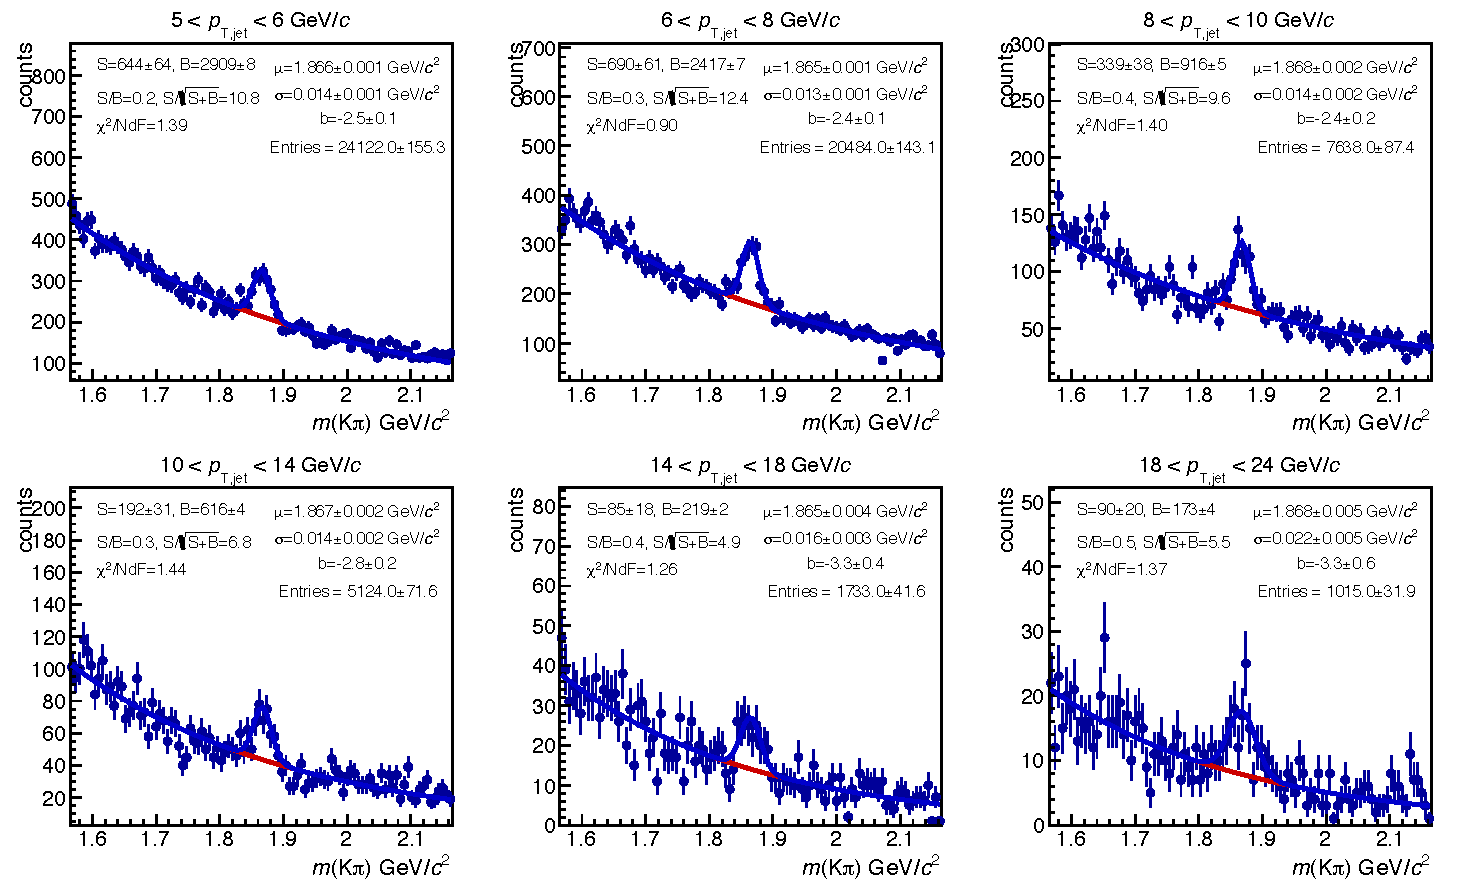
\includegraphics[width=1.0\textwidth]{img/InvMassSingleDiff}
 \caption{Invariant mass plots of \Dzero\ meson candidates found in \pp\ collisions at \s\ = 7 TeV. This analysis
 was performed on a sample of $3\times 10^8$ minimum-bias events. Each of the six plots shown includes \Dzero\ candidates
 with an associated jet \pt\ in the range printed above. Jets are reconstructed using the \antikt\ algorithm with resolution parameter $R=0.6$. } 
 \label{fig:InvMassSingleDiff}
\end{center}
\end{figure}
\subsubsection{Final corrections and systematic uncertainties}
Due to finite detector resolution, the spectrum obtained as outlined above is distorted. In addition the reconstruction efficiency is quite low
and \pt-dependent, especially for the D meson ($\epsilon_{D^0} \sim 10-20\%$, see Ref.~\cite{ALICE:2012d}). This is due both to the tracking efficiency ($\sim 80\%$, see Ref.~\cite{ALICE:2014b}),
which affects the probability of reconstructing the decay products, and to the topological cuts. These effects will be corrected for using a combination of Monte Carlo simulation and data-driven methods, currently being refined.
The corrections applied to remove or reduce effects due to detector resolution and efficiency are referred to as \emph{unfolding} and make use of modern statistical analysis methods~\cite{Hocker:1995, Dagostini:1995}.
A full \emph{closure} test using Monte Carlo simulated events is underway, to validate the ability of the analysis procedures to recover the signal.

Systematic uncertainties will be thoroughly assessed. Systematic uncertainties can arise from a variety of sources.
Some of the major sources come from irreducible inaccuracies in the assessment of the detector performance, in particular tracking efficiency, 
momentum resolution, primary/secondary vertex resolution, PID.
Other sources are more specific to the analysis procedures and are related to the invariant mass fits and to the unfolding techniques.

\subsection{Timeline}
I started working on this analysis in spring 2015, alongside with other service work activities for ALICE (see Section~\ref{sect:ServiceWork}).
My focus has been on developing the analysis techniques, which bring a number of novelties and challenges, as briefly outlined in the previous Section.
The analysis techniques are now quite solid and I have received positive feedback from the conveners of the physics analysis group (PAG) of the ALICE Collaboration,
where my analysis is reviewed. The last pieces that need some refinement are the unfolding procedures and corrections and the assessment of the systematic uncertainties.
I expect that it will take $\sim 6$ months to complete the analysis with the 7 TeV \pp\ collision data (collected in 2010) and write a paper draft for the Collaboration internal review (January 2017). Once approved
by the Collaboration the paper will be submitted to a peer-reviewed journal.
In the meantime I have submitted an abstract to the organizers of the \emph{Hot Quarks 2016 Workshop}~\cite{HotQuarks:2016}, which will be held in South Padre Island, TX, September 12-17. 
The abstract has been accepted and I plan to report on the analysis procedures and show partial results.

The extension of the analysis to the 8 TeV (2012) and 13 TeV (2016) \pp\ collision data will take an additional $\sim 6-12$ months. The major addition is the inclusion of the calorimeter
which will allow to perform a full jet reconstruction.
I will prepare another peer-reviewed paper in which these additional results will be reported.
I expect to graduate in May 2018.

\section{Service work}
\label{sect:ServiceWork}

\subsection{TPC upgrade for LHC Run-3}
The Relativistic Heavy Ion Group (RHIG) at Yale has taken a major role in the upgrade of the ALICE TPC~\cite{ALICE:2014c} for LHC Run-3 phase (scheduled to start in 2021).
A significant increase of the LHC luminosity for heavy ions is expected in Run-3, with collision rates of about 50 kHz. This implies a substantial enhancement
of the sensitivity to a number of rare probes that are key observables for the characterization of the QGP. In order to fully exploit this scientific potential, ALICE needs to
upgrade its detector to be able to cope with a much larger collision rate.

Currently the TPC read-out rate is limited both by the electronic read-out ($\sim 300$~Hz) and the \emph{gating grid} cycle ($\sim 3$~kHz).
The gating grid is used to trap the ions produced at the end-caps in the Multi-Wire Proportional Chambers (MWPCs), and prevents them from flowing back into the bulk of the TPC.
It operates by applying an appropriate electric potential just in front of the MWPCs. When the gate is in its \emph{closed} state
it becomes opaque to charged particles, preventing ions produced in the MWPCs from back-flowing, but also stopping
electrons from the bulk of TPC. This means that the the read-out rate is limited by the TPC gating grid cycle: $\sim 100\, \rm \mu s$
open to let electrons drift towards the MWPCs and $\sim 200\, \rm \mu s$ closed to stop all ions produced in the MWPCs.

The approach taken by the ALICE Collaboration is to replace the gating grid system and the MWPCs with Micro-Pattern Gas Detectors (MPGDs),
such as \emph{Gas Electron Multiplier} (GEM) detectors and \emph{Micromegas} detectors. These detectors show intrinsically low values for ion back-flow~\cite{Colas:2004,Sauli:2006},
which means that a gating grid is no longer required.

Throughout 2014, we have performed measurements at Yale on a small prototype of a gas chamber, which uses a stack of two GEMs and a Micromegas to amplify the ionization
produced by a small radioactive source. In November 2014, a larger prototype was also shipped to CERN, where we performed another set of measurements using
the Proton Synchrotron (PS) and Super-Proton-Synchrotron (SPS) beam facilities.
The results of these measurements have been included in the Addendum to the ALICE TPC Upgrade Technical Design Report~\cite{ALICE:2015b}.
In addition we have submitted a paper~\cite{Aiola:2016a} to \emph{Nuclear Instrument and Methods}, which is currently being reviewed by the editor.

The ALICE Collaboration and the CERN management have approved the TPC upgrade and we have now moved into the production phase.
The Yale group is leading the construction and commissioning of the Inner Read-Out Chambers (IROCs) of the TPC using facilities and labs on the Yale campus.

\subsection{The EMCal-DCal 2016 trigger commissioning}
\label{sect:TriggerCommisioning}
At the LHC, the interaction rate is much higher than the maximum read-out rate supported by the experiments. As a consequence only a fraction of the collisions delivered
by the LHC can be read-out and recorded by ALICE. The \emph{minimum bias trigger} is typically \emph{downscaled}, i.e. only a fraction of collisions
that fulfill the trigger condition are actually read-out. In the case of downscaling, collisions are skipped randomly. This is however not very efficient
if one wants to look at rare physics processes, such as a hard scattering. A \emph{rare trigger} implements more elaborate conditions to select events that 
potentially include rare processes. This allows to sample a larger luminosity, at the expense of introducing a bias in the event sample. It is important
to be able to control and understand the trigger bias and the trigger inefficiencies for each particular process being analyzed. This is usually done
using a combination of data driven methods (that typically rely on a large enough \emph{minimum bias} sample) as well as Monte Carlo simulations.

\begin{figure}[tb]
\begin{center}
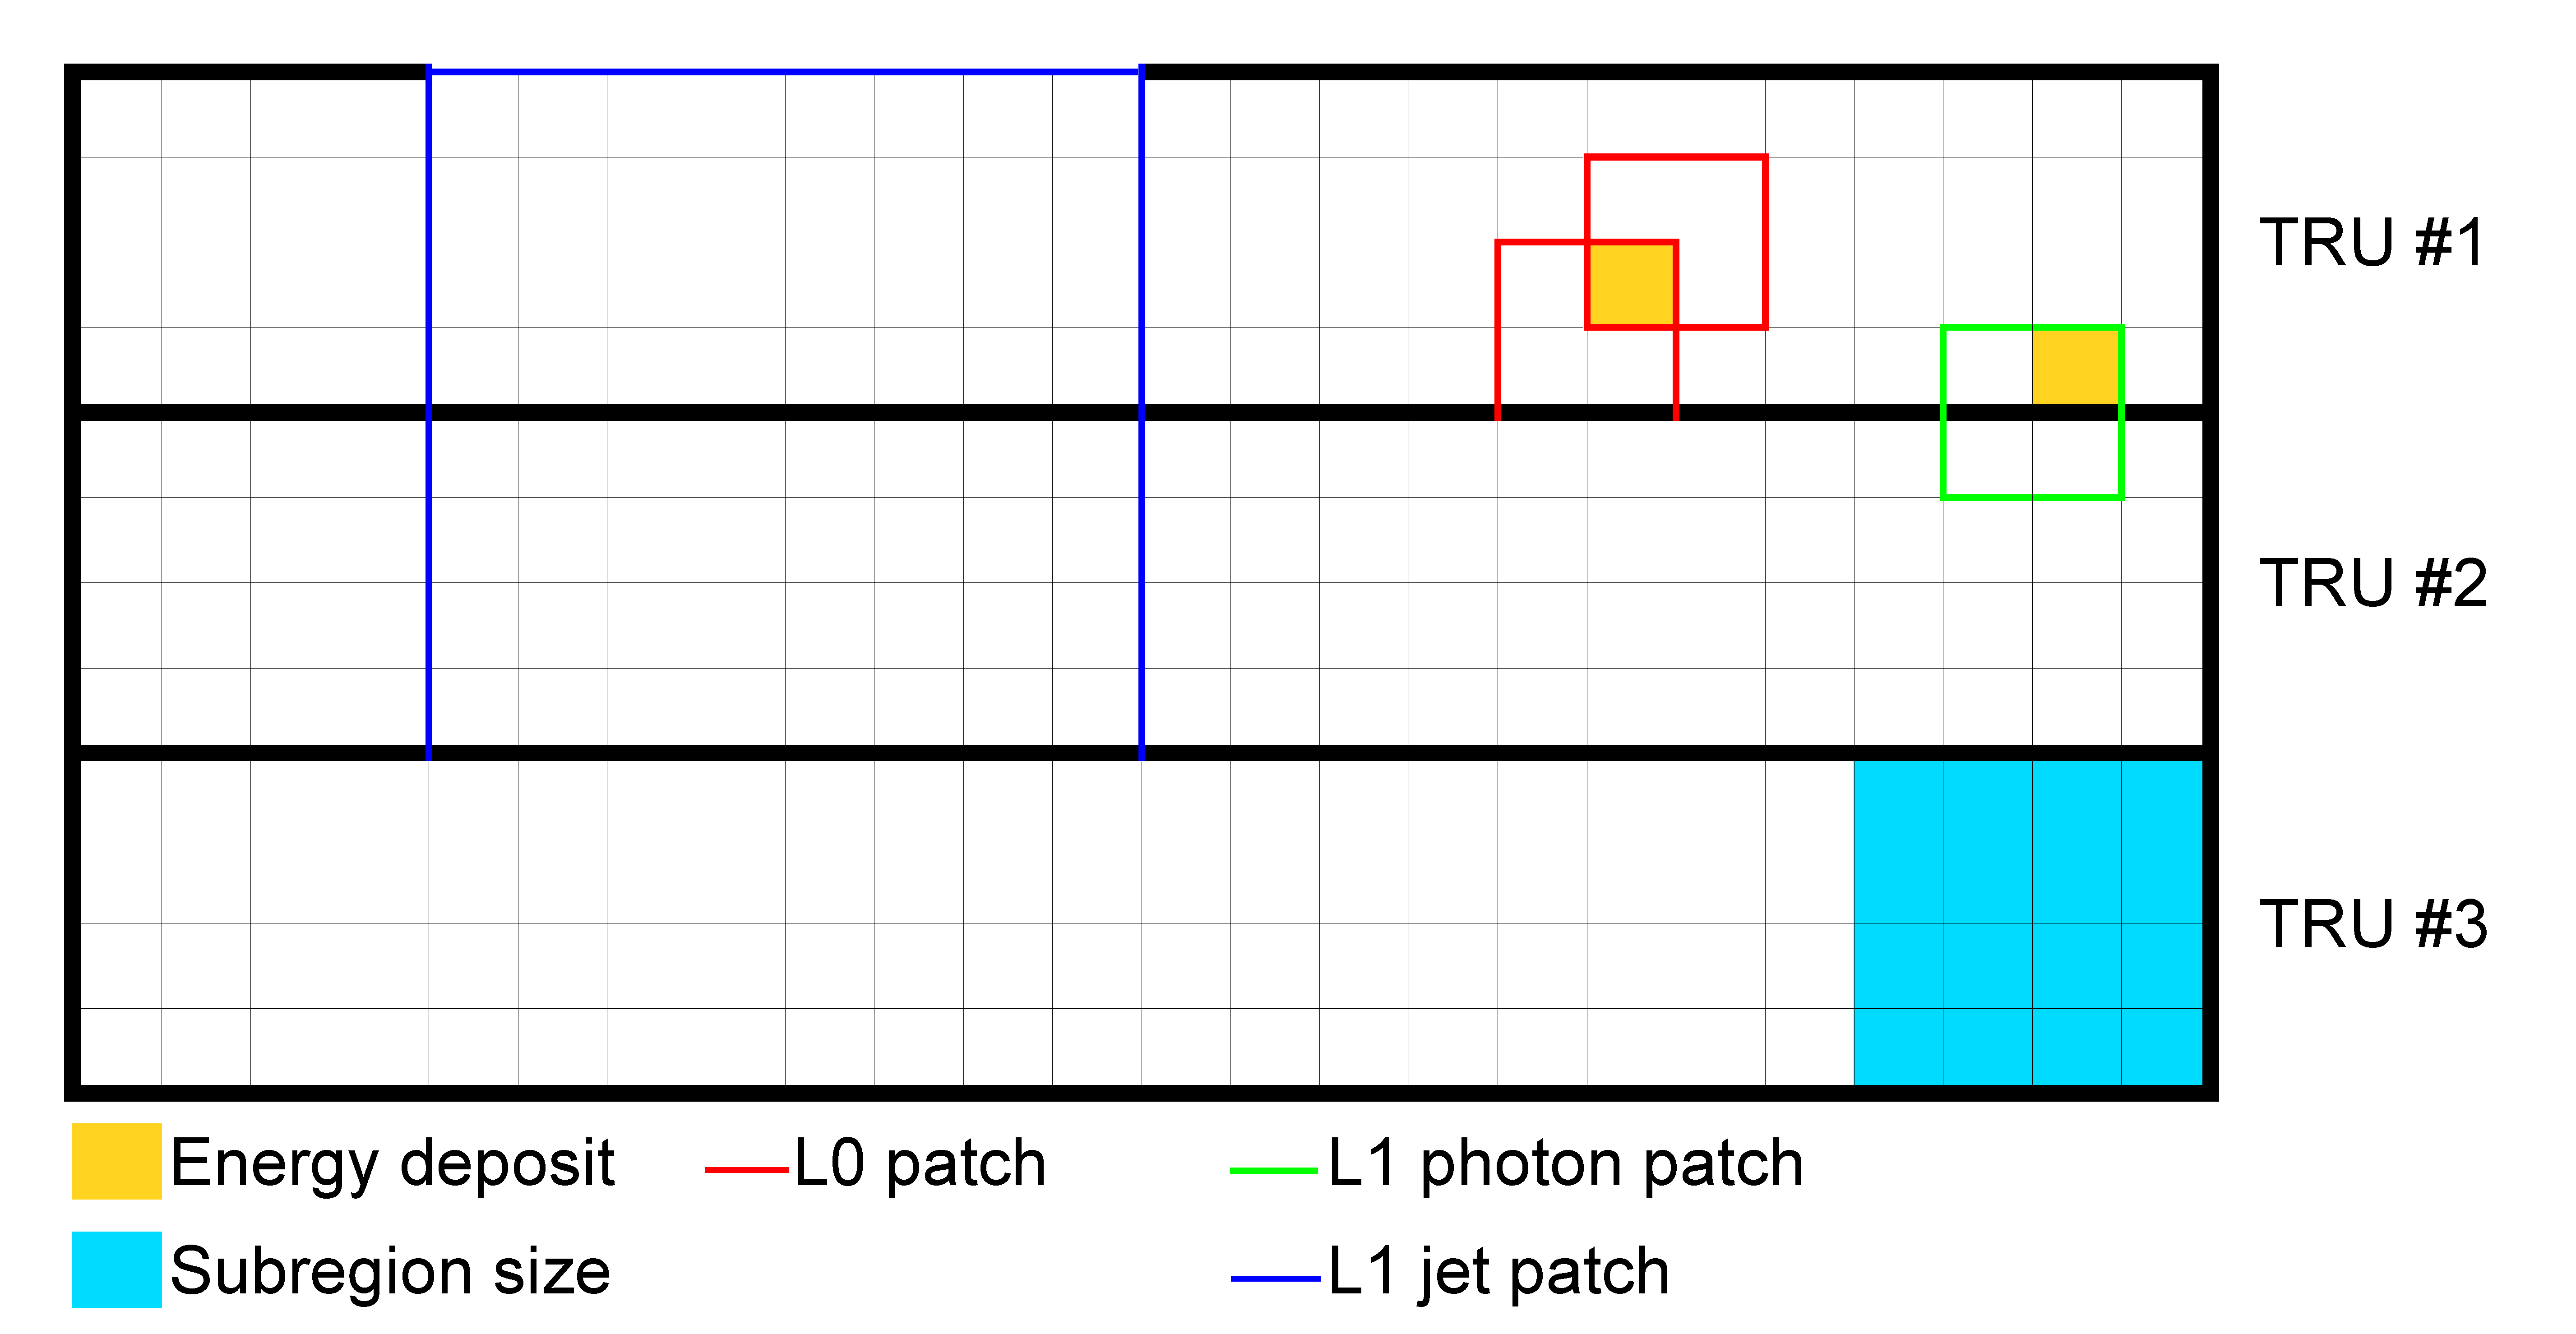
\includegraphics[width=0.6\textwidth]{img/emcaltrigger}
 \caption{View of a full EMCal super-module. The thick lines divide different TRU. The light lines represent 2x2 towers each, which is the smallest unit
available for trigger decisions.} 
 \label{fig:emcaltrigger}
\end{center}
\end{figure}
Both the EMCal and DCal can provide rare triggers. ALICE has implemented two levels of triggers: the Level-0 (L0) which provides a decision within 
$0.9\,\rm \mu s$ and the Level-1 (L1) which provides a decision within $6.5\,\rm \mu s$ after L0~\cite{ALICE:2014b}. The L0 EMCal-DCal trigger algorithm looks for a high energy
deposition scanning the acceptance in 4x4 tower windows. This scan is performed separately in each Trigger Region Unit (TRU) which corresponds to 1/3 of a EMCal-DCal super-module.
A 4x4 window is relatively small and can therefore trigger on contained showers of single electrons, photons or \pizero.
In order to identify events containing larger showers, such as the ones initiated by a jet, we need to scan the acceptance using a larger window. This is possible using
L1 triggers that can take decisions based on the information coming from the entire calorimeter acceptance rather than a single TRU. The EMCal-DCal implements two L1 algorithms
which differ essentially only in the size of the trigger window: 4x4 for the L1 \emph{gamma} algorithm, used for electrons, photons and \pizero, and 32x32 (or 16x16) for the L1 \emph{jet} algorithm.
Figure~\ref{fig:emcaltrigger} is visual representation of the L0 and L1 trigger algorithms.

\begin{figure}[tb]
\begin{center}
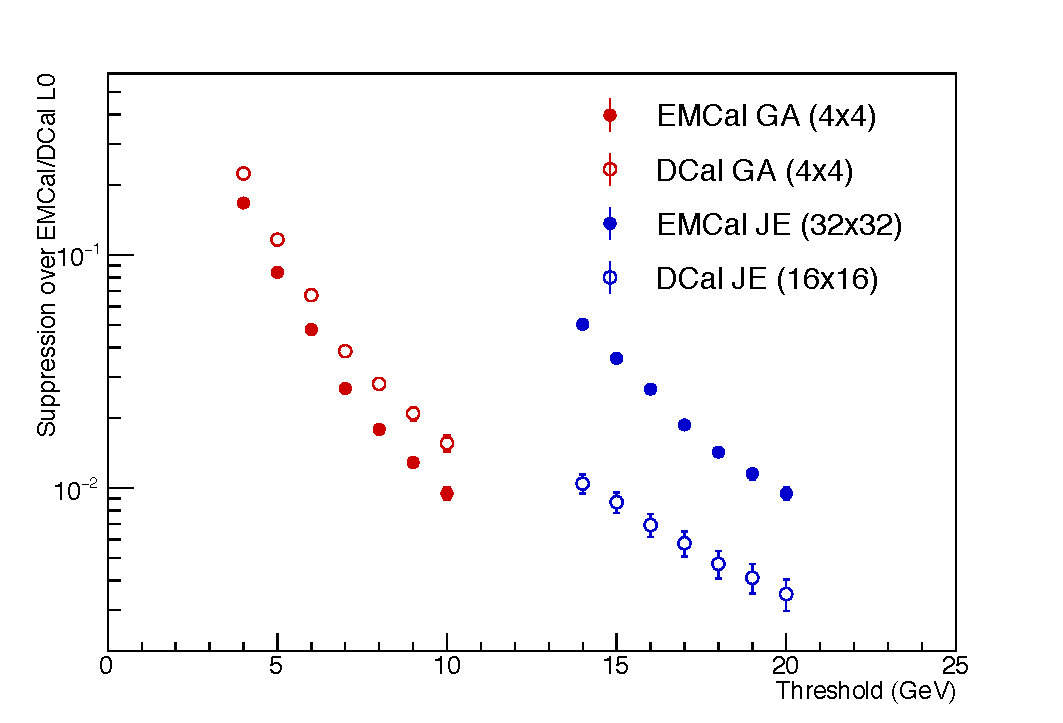
\includegraphics[width=0.8\textwidth]{img/EMCalTriggerSuppression}
 \caption{Suppression of the L1 trigger rate over the L0 rate as a function of thresholds for different trigger algorithms (gamma in red and jet in blue) 
 and different detectors (EMCal in solid symbols and DCal in open symbols). This analysis was performed using data collected during the first few weeks of
 \pp\ collisions at \s\ = 13 TeV in the spring 2016.} 
 \label{fig:EMCalTriggerSuppression}
\end{center}
\end{figure}
In the spring 2016 I spent a couple of months at CERN helping with the commissioning of the L1 triggers, as well as with general operations of the EMCal-DCal during data taking.
In particular my contribution is related to the fine tuning of the trigger thresholds for the L1 gamma and jet algorithms. The thresholds are set according to the physics goals discussed
and approved by the different working groups of the Collaboration. The triggers need also to provide a suppression compatible with the ALICE maximum read-out rate.
Figure~\ref{fig:EMCalTriggerSuppression} shows the suppression provided by the L1 gamma and jet algorithms over the L0 triggered events (with a L0 threshold set at 2.5~GeV), separately for EMCal and DCal.

\bibliography{biblio}{}
\bibliographystyle{utphys}

\end{document}
